\section{RTM Algorithm and Analysis}

As it is mentioned in the previous section that the Reverse Time Migration
algorithm can gain a big improvement but it is computationally demanding.
In this section, we have a look at the detail of the algorithm and present
a computation complexity analyze of it.

The main steps of the algorithm is explained as below\cite{rtm}.

\begin{enumerate}
\item the forward extrapolation of a modelled source waved for each shot
  location through a gridded velocity model is performed. And the wave
  field at each time step is saved for later application of the ``imaging
  condition''.
\item the receiver wave field for each shot, which is recorded in the
  field, is backward propagated in time through the same velocity model.
\item at each time step, the corresponding source and receiver wave fields
  are correlated by applying the imaging condition. Thus, the final
  wave field in the source propagating scheme is correlated with the
  initial wave field in the receiver propagation scheme, and so on backward
  through the receiver propagation.
\item the result are summed to form a partial image volume for each shot.
\item the image volumes for consecutive gathers are spatially summed to
  produce the final pre-stack depth image.
\end{enumerate}

So, now you may know why RTM is so computation expensive and has several
decades to be commercially implemented.

\subsection{Mathematical Derivation of RTM}

If we assume that the wave that the wave injects is acoustic wave (sound
wave), then we can use the acoustic wave equation (\ref{eq:acoustic}) as
the first step of the derivation.

\begin{equation}
  \frac{\partial ^2u}{\partial t^2}=c^2 \cdot \left(  \bigtriangledown ^2u \right) +s
  \label{eq:acoustic}
\end{equation}

where \( u = u(x, y, z, t) \) is the pressure field, \(c = c(x, y, z) \) is
the velocity field, \( s = s(x, y, z, t) \) is the source term, and \(
\bigtriangledown ^2 \) is the three dimensional Laplace operator.

The Laplace operator is a second order differential operator in the n-dimensional
Euclidean space, defined as the divergence (\( \bigtriangledown \)) of the gradient
(\( \bigtriangledown f\)). Thus if \( f \) is a twice-differentiable real-valued
function, then the Laplacian of \( f \) is defined by

\[
  \bigtriangleup f = \bigtriangledown ^2 f = \bigtriangledown \cdot
  \bigtriangledown f
\]

Equivalently, the Laplacian of \( f \) is the sum of all the unmixed second
partial derivatives in the Cartesian coordinates:

\[
  \bigtriangleup f = \sum _{i=i} ^n \frac{\partial ^2 f}{\partial x_i ^2}
\]

In particular, if the variable x, y and z denote the three dimensional
Cartesian coordinates, the expansion is:

\begin{equation}
  \bigtriangleup f  = \bigtriangledown ^2 f = \frac{ \partial ^2 f}{\partial x^2} +
                     \frac{ \partial ^2 f}{\partial y^2} +
                     \frac{ \partial ^2 f}{\partial z^2}
  \label{eq:laplacian}
\end{equation}

Thus, replace the Laplacian operator with (\ref{eq:laplacian}), the
equation (\ref{eq:acoustic}) could be derived as:

\begin{equation}
  \frac{\partial ^2u}{\partial t^2}=
  c^2\cdot\left(
  \frac{ \partial ^2 u}{\partial x^2} +
  \frac{ \partial ^2 u}{\partial y^2} +
  \frac{ \partial ^2 u}{\partial z^2}
  \right)
  +s
  \label{eq:acoustic2}
\end{equation}

Equation (\ref{eq:acoustic2}) can be further factored as:
\begin{equation}
  \frac{u_{t+1} - 2u_{t} + u_{t-1}}{dt^2}=
  c^2\left(
  \frac{ \partial ^2 u}{\partial x^2} +
  \frac{ \partial ^2 u}{\partial y^2} +
  \frac{ \partial ^2 u}{\partial z^2}
   \right)
  +s
  \label{eq:acoustic3}
\end{equation}

Then we introduce a method called \emph{stencil}, which is a geometric
arrangement of a nodal group that relate to the point of interest by using
a numerical approximation routine in mathematics, especially the areas of
numerical analysis concentrating on the numerical solution of partial
differential equations. The derivation of stencil from the second order
partial difference is in appendix. Now, equation (\ref{eq:acoustic3}) could
be written as:

\begin{equation}
  \frac{u_{t+1} - 2u_{t} + u_{t-1}}{dt^2}=
  c^2 \cdot\left( \frac{1}{dh^2} \cdot stencil\left( p_t \right) \right)
     +s
  \label{eq:acoustic4}
\end{equation}

where \( dh \) is the distance between the two neighbours of the stencil
operation. For a specific point x, the stencil result of that point in 6th
order is:

\begin{equation}
  \begin{split}
    {f(x)}'' =
    & w_{-3}f\left( x - 3 \Delta x \right) +
      w_{-2}f\left( x - 2 \Delta x \right) +
      w_{-1}f\left( x - \Delta x   \right) + \\
    & w_{0}f\left( x \right) + \\
    & w_{1}f\left( x + \Delta x \right) +
      w_{2}f\left( x + 2 \Delta x \right) +
      w_{3}f\left( x + 3 \Delta x \right)
  \end{split}
\end{equation}

where \( \Delta x \) has the same meaning with \( dh \) in equation
\ref{eq:acoustic4}. To give a better vision, Figure
\ref{fig:6th_order_stencil_1d} give a outline of one dimensional stencil.

\begin{figure}[h]
  \centering
  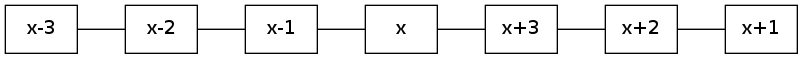
\includegraphics[scale=0.4]{img/6th_order_stencil.png}
  \caption{6th order one dimensional stencil}
  \label{fig:6th_order_stencil_1d}
\end{figure}

Figure (\ref{fig:6th_order_stencil_1d}) give us a array like presentation of
1D stencil, and the result at element i is:

\[
  y\left[ i \right] = c_3  x\left[ i-3 \right] +
                      c_2  x\left[ i-2 \right] +
                      c_1  x\left[ i-1 \right] +
                      c_0  x\left[ i \right] +
                      c_1  x\left[ i+1 \right] +
                      c_2  x\left[ i+2 \right] +
                      c_3  x\left[ i+3 \right];
\]

where \( c_0 \) to \( c_3 \) are dedicated coefficients based on the
different order of the stencil.

In the previous acoustic equation, the stencil is a 6th order 3D stencil,
which is denoted by x, y and z axis. Thus, given a point (x, y, z), there
are 18 (3 x 6) points around and the center point, 19 points altogether,
will be used to perform the calculation. Figure
(\ref{fig:6th_order_stencil_3d}) gives a sketch of such stencil.

\begin{figure}[h]
  \centering
  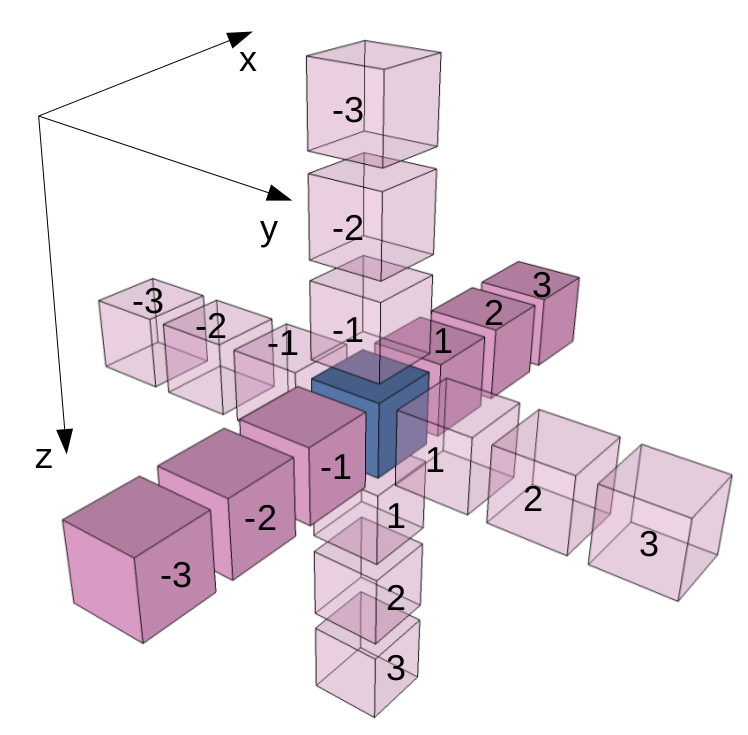
\includegraphics[scale=0.4]{img/stencil_6_3d.png}
  \caption{6th order 3 dimensional stencil}
  \label{fig:6th_order_stencil_3d}
\end{figure}

The calculation of the stencil in Figure (\ref{fig:6th_order_stencil_3d})
is sum of the x, y and z axis. We can draw a formula to denote it.

\begin{equation}
  g(x,y,z) = \sum _{i=-3} ^{+3} w_i  f(i,y,z) +
             \sum _{j=-3} ^{+3} w_j  f(x,j,z) +
             \sum _{k=-3} ^{+3} w_k  f(x,y,k) -
             2f(x,y,z)
 \label{eq:stencil_3d}
\end{equation}

Changing the equation (\ref{eq:stencil_3d}) to the programming psudo-code
is very convenient for programming to code. Listing (\ref{lst:stencil_code_1element})
shows the desired psudo-code.

\begin{figure}
\centering
\lstinputlisting[
  caption={Pseudo code of calculating one element using stencil method},
  label={lst:stencil_code_1element}
  ]
  {code/stencil_1elem.c}
\end{figure}

Listing (\ref{lst:stencil_code_1element}) only works for 1 element in the
array. In practice and in the previous equation (\ref{eq:acoustic}), all
the elements in the three dimension volume should be calculated one by one
except for the boundaries. Thus the complexity of calculating the stencil
in a volume is \BigO{n^3} 
\subsection{Complexity analyze}

Dablain (1986) effectively applies explicit high-order finite
difference spatial derivatives to the acoustic wave equation.
We also apply high-order spatial derivatives to the acoustic
wave equation. Using the \( 2^{nd} \) in space finite differences, the
forward and backward wave field propagations can be calculated as
\cite{rtm_psdm}:

\begin{equation}
  u ^{l(+/-)1} _{i,j,k} = 2u^l _{i,j,k} - u^{l(+/-)1} _{i,j,k} + \Delta t^2
  c^2 _{i,j,k} (\left( \bigtriangledown ^2 u ^l _{i,j,k}  \right) ^ n_0 +
  s ^l _{i,j,k})
\end{equation}

where

\[u^l _{i,j,k} = u(i\Delta x, j \Delta y, k \Delta z, l \Delta t),\]
\[ s^l _{i,j,k} = s(i\Delta x, j \Delta y, k \Delta z, l \Delta t),\]
\[ c_{i,j,k} = u(i\Delta x, j \Delta y, k \Delta z), \]

and \( \Delta t \) =  the temporal step size for finite differencing, \(
\Delta x \), \( \Delta y \), and \( \Delta z \) are the spatial sampling
intervals, and \( \bigtriangledown ^2 u^t _{x, y, z} \) the Laplacian
calculated with \( n^{th} \) order of accuracy at each time step t,
centered at an x-, y-, and z- location. During the backward extrapolation
the source
term is replaced by the recorded input data. The Laplacian with
\( n^{th} _0 \) order accuracy can be given by ().

\begin{equation}
  (\bigtriangledown ^2 u ^l _{i,j,k})^n_0 = w_0(\frac{1}{\Delta x^2} +
  \frac{1}{\Delta y^2} + \frac{1}{\Delta z^2})u^l _{i, j, k} + \Phi
\end{equation}

where

\begin{equation}
  \begin{split}
    \frac{\Phi}{\sum_{m=1} ^{n_0 / 2}w_m} =
      &\frac{1}{\Delta x^2}\left(u^l _{i-m, j, k}+ u ^l _{i+m, j, k}
      \right) + \\
      &\frac{1}{\Delta y^2}\left(u^l _{i, j-m, k}+ u ^l _{i, j+m, k}
      \right) + \\
      &\frac{1}{\Delta x^2}\left(u^l _{i, j, k-m}+ u ^l _{i, j, k+m} \right)
  \end{split}
\end{equation}

where w are finite differencing coefficients of the desire
accuracy. Coefficients are calculated via a series expansion
method. For example, if a second derivative of a function
\( f(x) \) is required to be approximated with \( 6^{th} \) order accuracy
on a uniform grid, the approximation can be written as:

\begin{equation}
  \begin{split}
    {f(x)}'' =
    & w_{-3}f\left( x - 3 \Delta x \right) +
      w_{-2}f\left( x - 2 \Delta x \right) +
      w_{-1}f\left( x - \Delta x   \right) + \\
    & w_{0}f\left( x \right) + \\
    & w_{1}f\left( x + \Delta x \right) +
      w_{2}f\left( x + 2 \Delta x \right) +
      w_{3}f\left( x + 3 \Delta x \right)
  \end{split}
  \label{eq:finite}
\end{equation}

Finite difference weights in (\ref{eq:finite}) can be calcuated using a
series expansion method. The coefficients are symmetrical around \( w_0 \)
for a uniform grid.

The cost of the method is approximately given by the following equation:

\begin{equation}
  C_e \approx 2n_t n_x n_y n_z \left( 3n_0 + 19 \right)
\end{equation}

Where \( C_e \) is the number of floating point operations; \( n_t \) is
the number of time steps; \( n_x , n_y , n_z \) are the number of samples
in the x, y and z directions.
